\usepackage{etex} %эта магическая херь избавляет от переполнения регистров TeX а!!!

\mode<article>{\usepackage{fullpage}}
\mode<presentation>{
    \usetheme{Madrid}
    \useoutertheme{shadow}
} 

\usepackage[utf8]{inputenc}
\usepackage[russian]{babel}
\usepackage{indentfirst}
\usepackage{graphicx}

\usepackage{amsmath}
\usepackage{amsfonts}
\usepackage{amsthm}
%\usepackage{algorithm}
%\usepackage{algorithmic}

%\usepackage[all]{xy}

\date{Лекция по дисциплине <<методы и средства защиты компьютерной информации>> (\today)}
\author[М.~М.~Шихов]{Михаил Шихов \\ \texttt{\underline{m.m.shihov@gmail.com}}}

%%для рисования графов пакетом xy-pic
%\entrymodifiers={++[o][F-]}

%%для псевдокода алгоритмов (algorithm,algorithmic)
%\renewcommand{\algorithmicrequire}{\textbf{Вход:}}
%\renewcommand{\algorithmicensure}{\textbf{Выход:}}
%\renewcommand{\algorithmiccomment}[1]{// #1}
%\floatname{algorithm}{Псевдокод}

%\setbeamercolor{alerted text}{fg=-green} %gyan, blue, green, -green

\title[Разделение секрета]{Разделение секрета и распределение ключей}

\newcommand{\Alice}{\textit{Алиса}}
\newcommand{\Bob}{\textit{Боб}}
\newcommand{\Clark}{\textit{Кларк}}

\begin{document}


\mode<article>{\maketitle\tableofcontents}

\frame<presentation>{\titlepage}
\begin{frame}<presentation>[allowframebreaks]
    \frametitle{Содержание}
    \tableofcontents
\end{frame}


\section{Протоколы распределения ключей симметричной схемы}


\subsection{Ключи}


Особенности симметричной схемы предполагают, что для безопасного обмена информацией между $n$ абонентами потребуется $\binom{n}{2}=\frac{n\cdot (n-1)}{2}$. Поэтому прибегают к схеме с доверенным лицом $S$: распределяется $n$ ключей $k_{S,i}$ между абонентом $1\leq i\leq n$ и доверенным лицом, а для получения \alert{сеансового} ключа для секретного обмена данными между абонентами используют протоколы распределения сеансового ключа через доверенное лицо. Распределенный сеансовый ключ обычно используется либо в течение единственного сеанса связи, либо в течение некоторого (относительно короткого) интервала времени.


\begin{frame}
    \frametitle{Ключи}
    
    \begin{itemize}
        \item Общее количество ключей для безопасного обмена между $n$ абонентами
        \[\binom{n}{2}=\frac{n\cdot (n-1)}{2}.\]
        \item Вводя доверенное лицо $S$, распределяют лишь $n$ \alert{долговременных} ключей $k_{S,i}$ между доверенным лицом $S$ и каждым $i$-м абонентом. $1\leq i\leq n.$
        \item Для секретного обмена между абонентами $i,j$ используется \alert{сеансовый} ключ $k_{i,j}$, распределяемый с помощью доверенного лица $S$.
    \end{itemize} 
\end{frame}


\subsection{Протоколы распределения сеансовых ключей}


\begin{frame}
    \frametitle{Протокол широкоротой лягушки}
    
    \begin{figure}
        \begin{center}
            \mode<presentation>{ 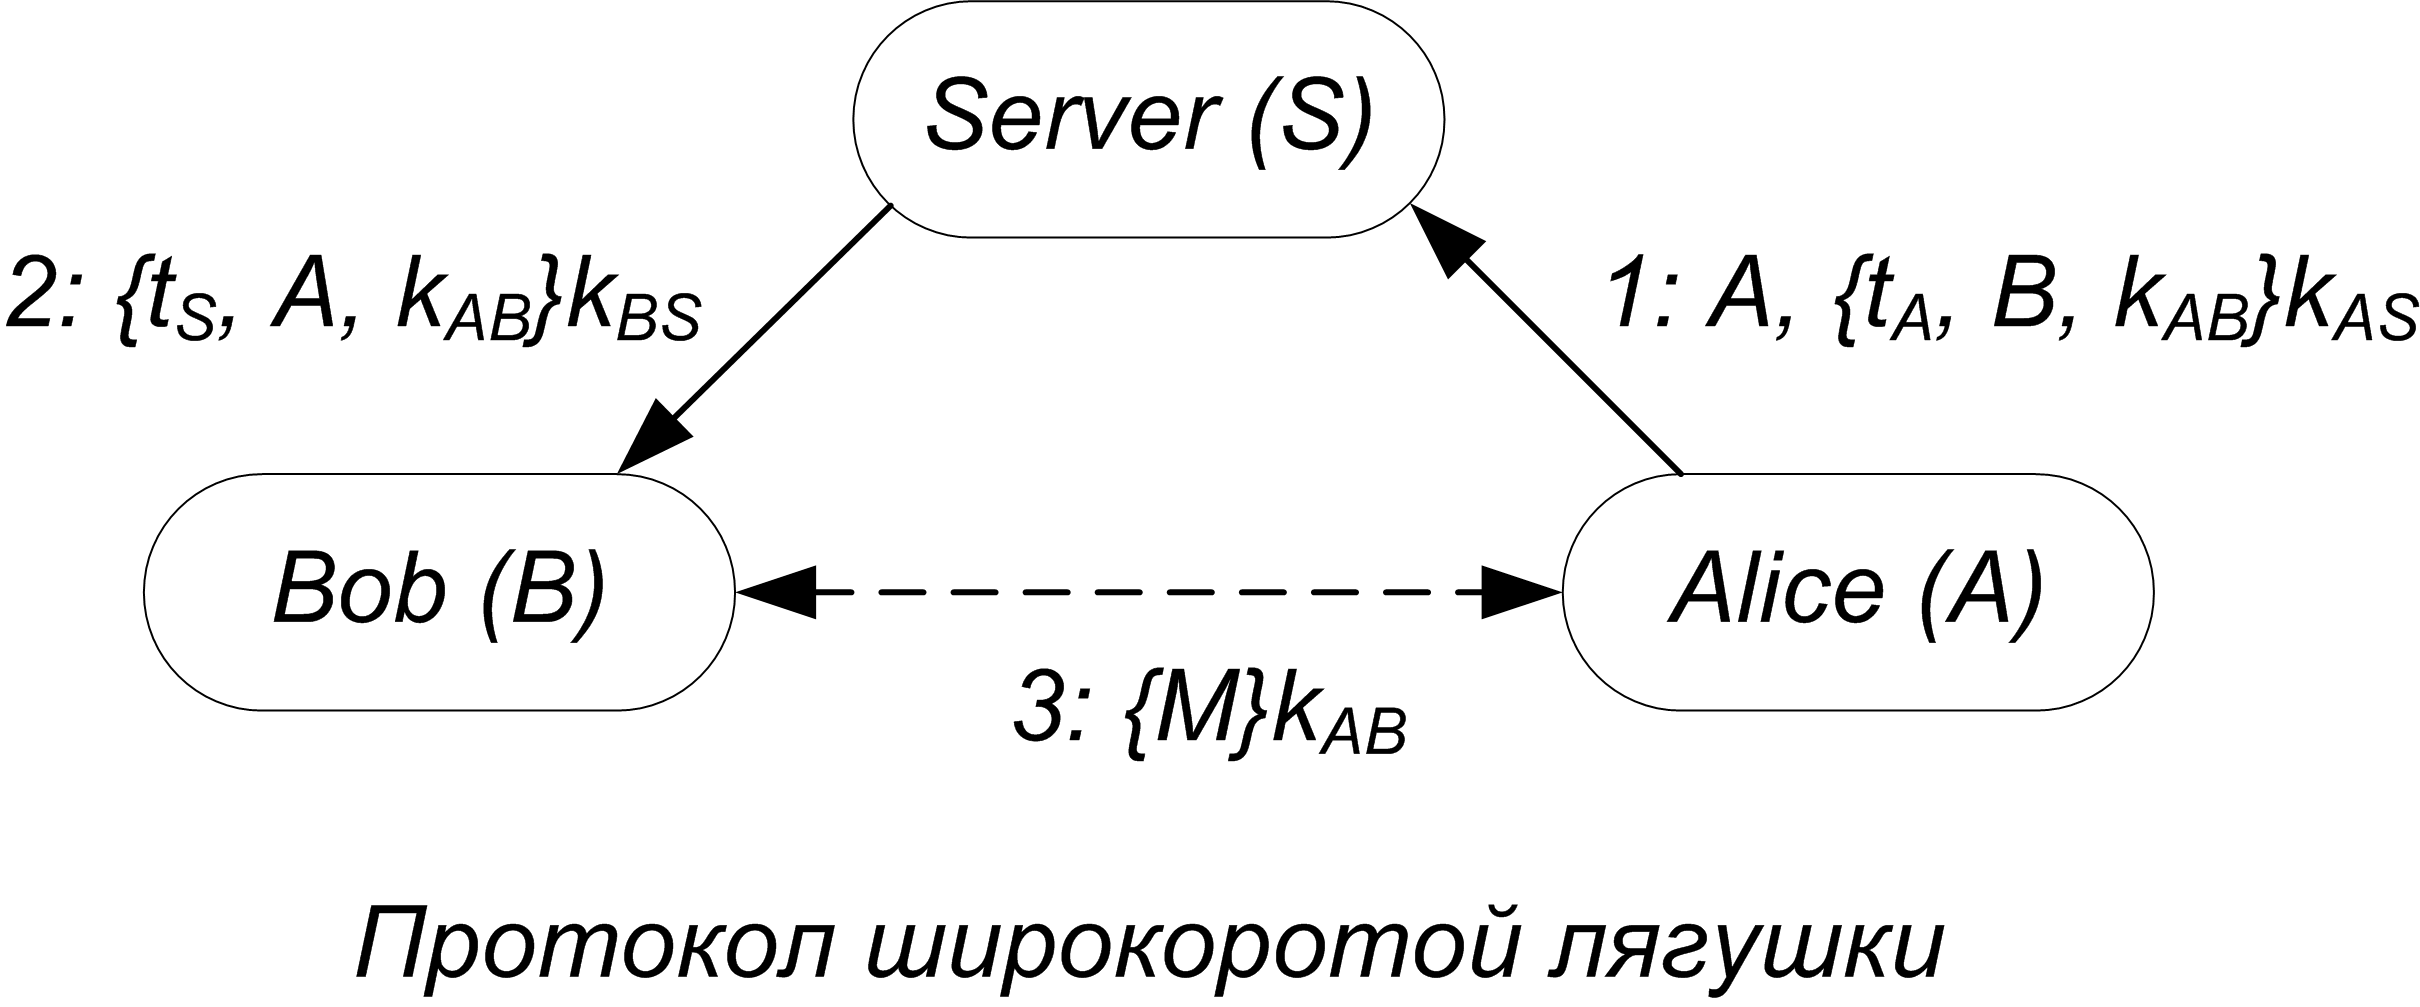
\includegraphics[width=.98\textwidth]{pict/frog} }
            \mode<article>{ 
                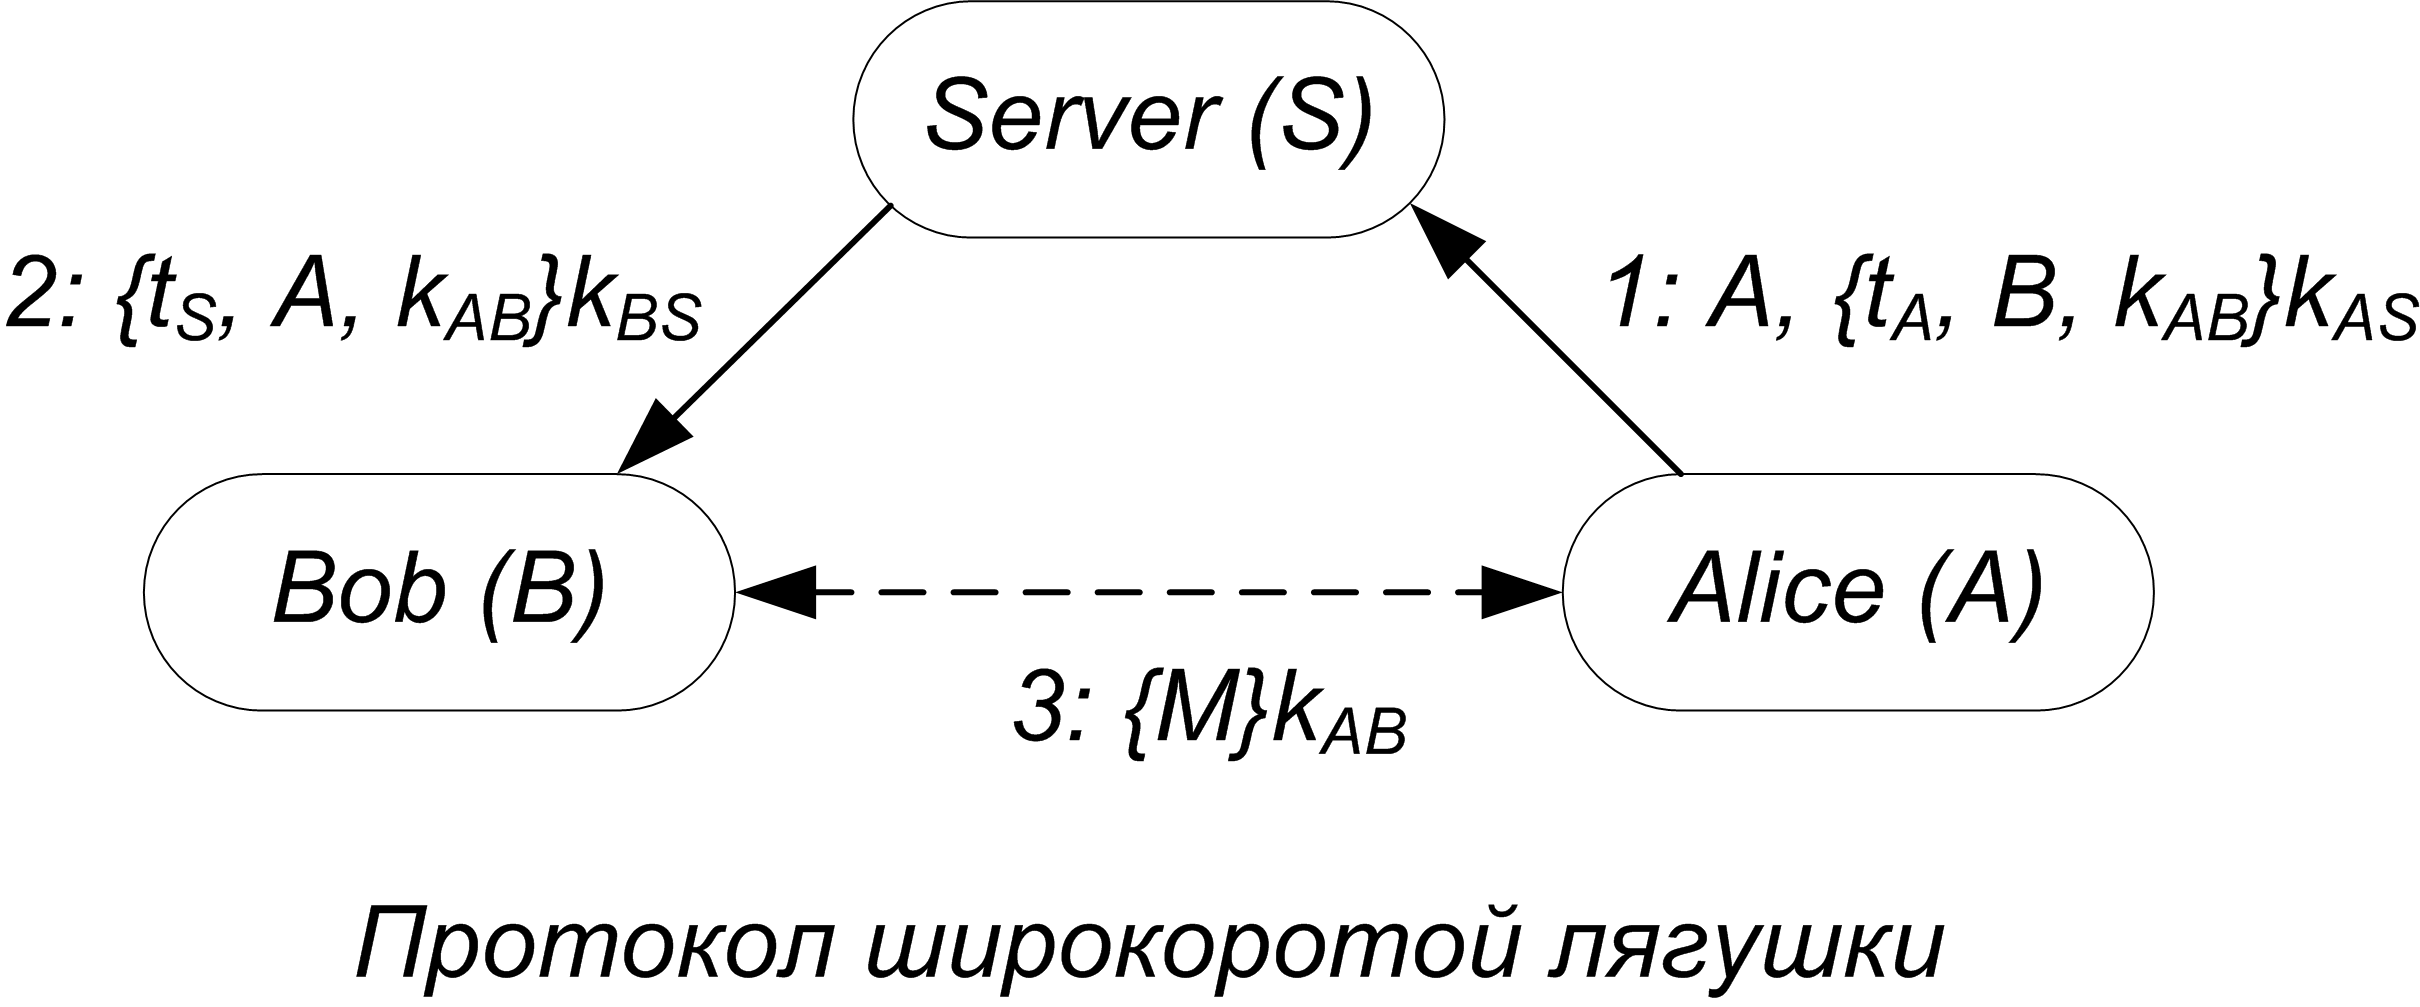
\includegraphics[width=.8\textwidth]{pict/frog}  
                \caption{Протокол широкоротой лягушки}\label{pict:frog}
            }
        \end{center}
    \end{figure} 
    \mode<article>{см. рис. \ref{pict:frog}}
\end{frame}


\begin{frame}
    \frametitle{Протокол Нидхема-Шредера}
    
    \begin{figure}
        \begin{center}
            \mode<presentation>{ 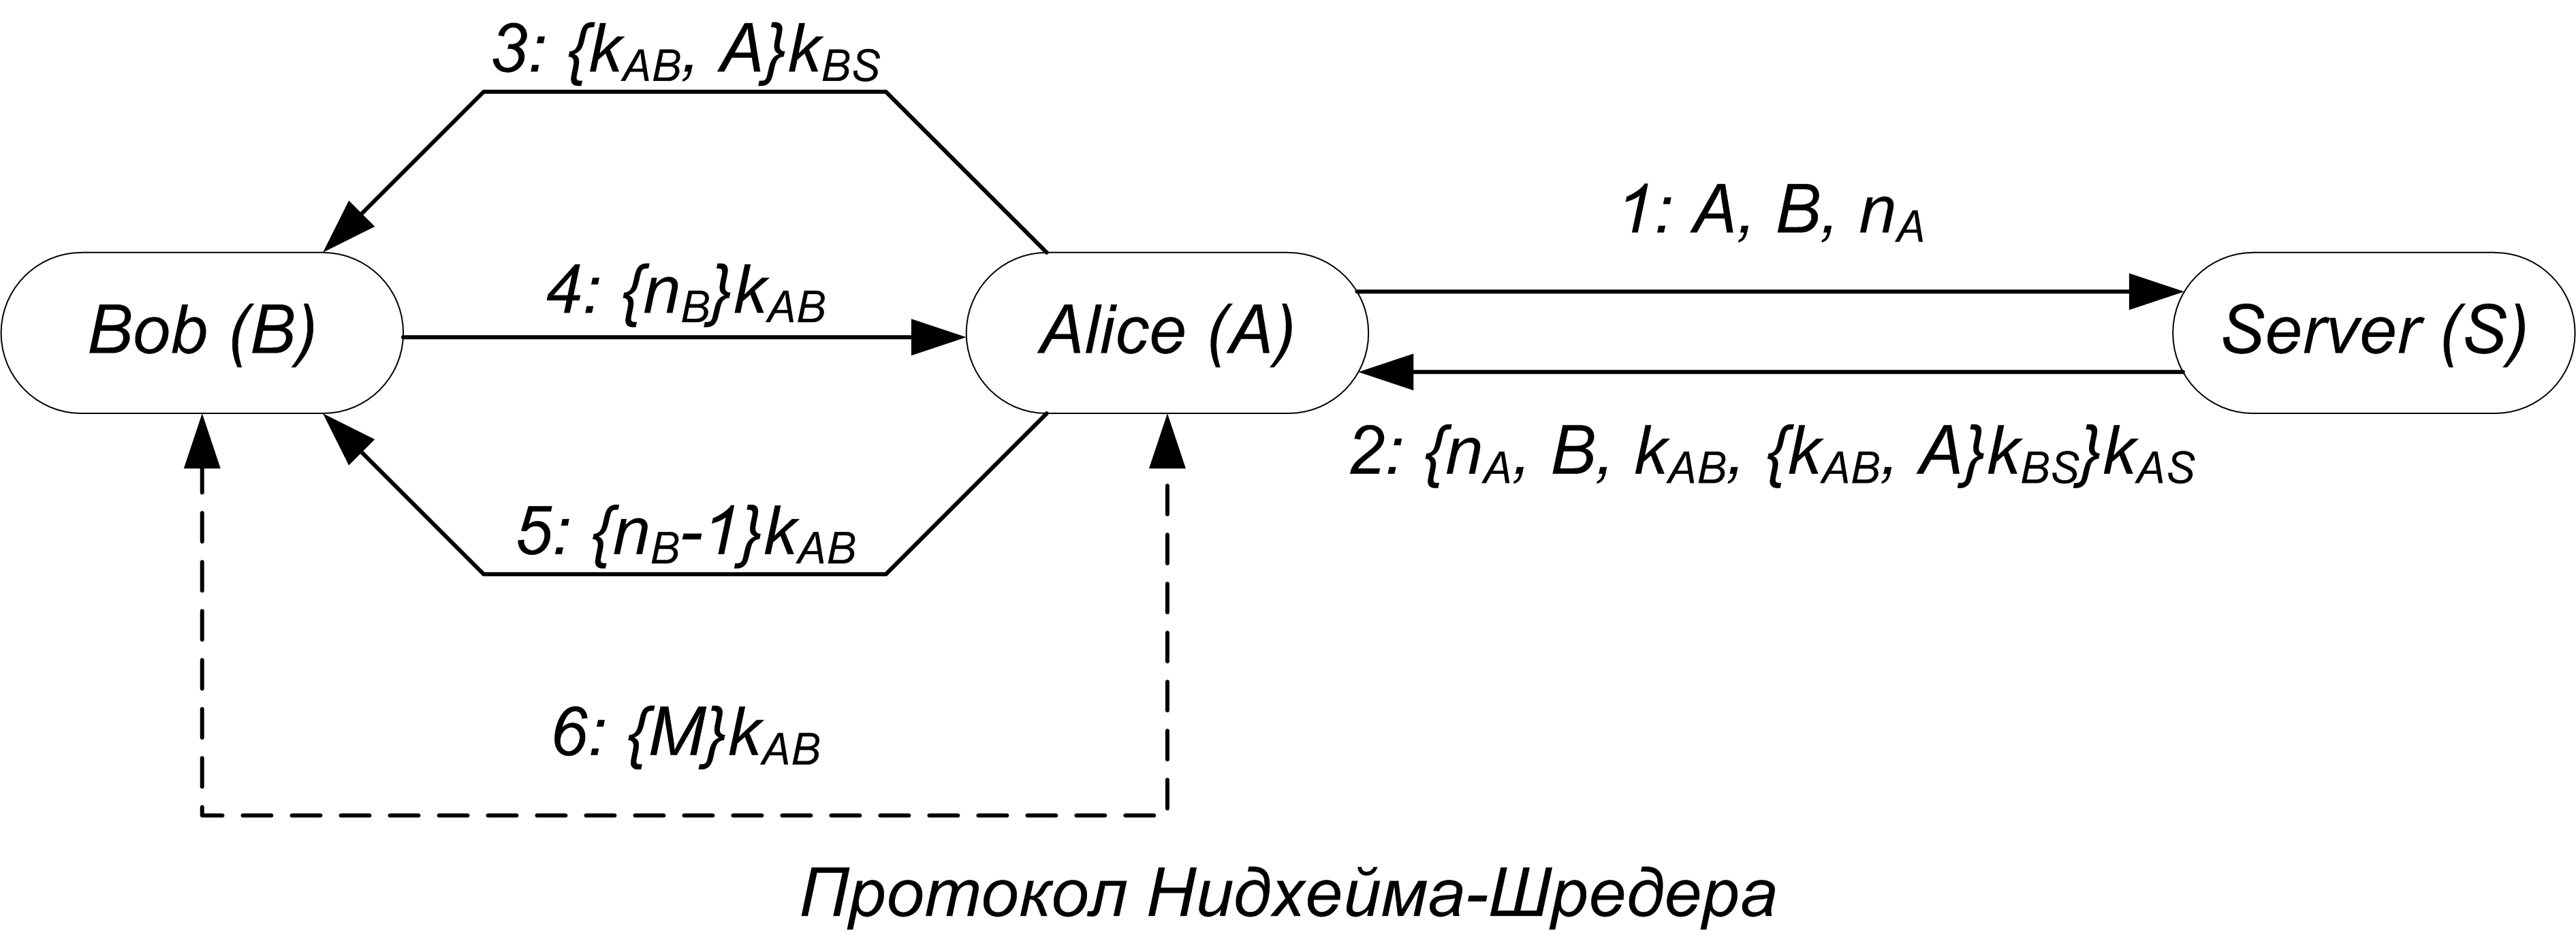
\includegraphics[width=.98\textwidth]{pict/nidhamshreder} }
            \mode<article>{ 
                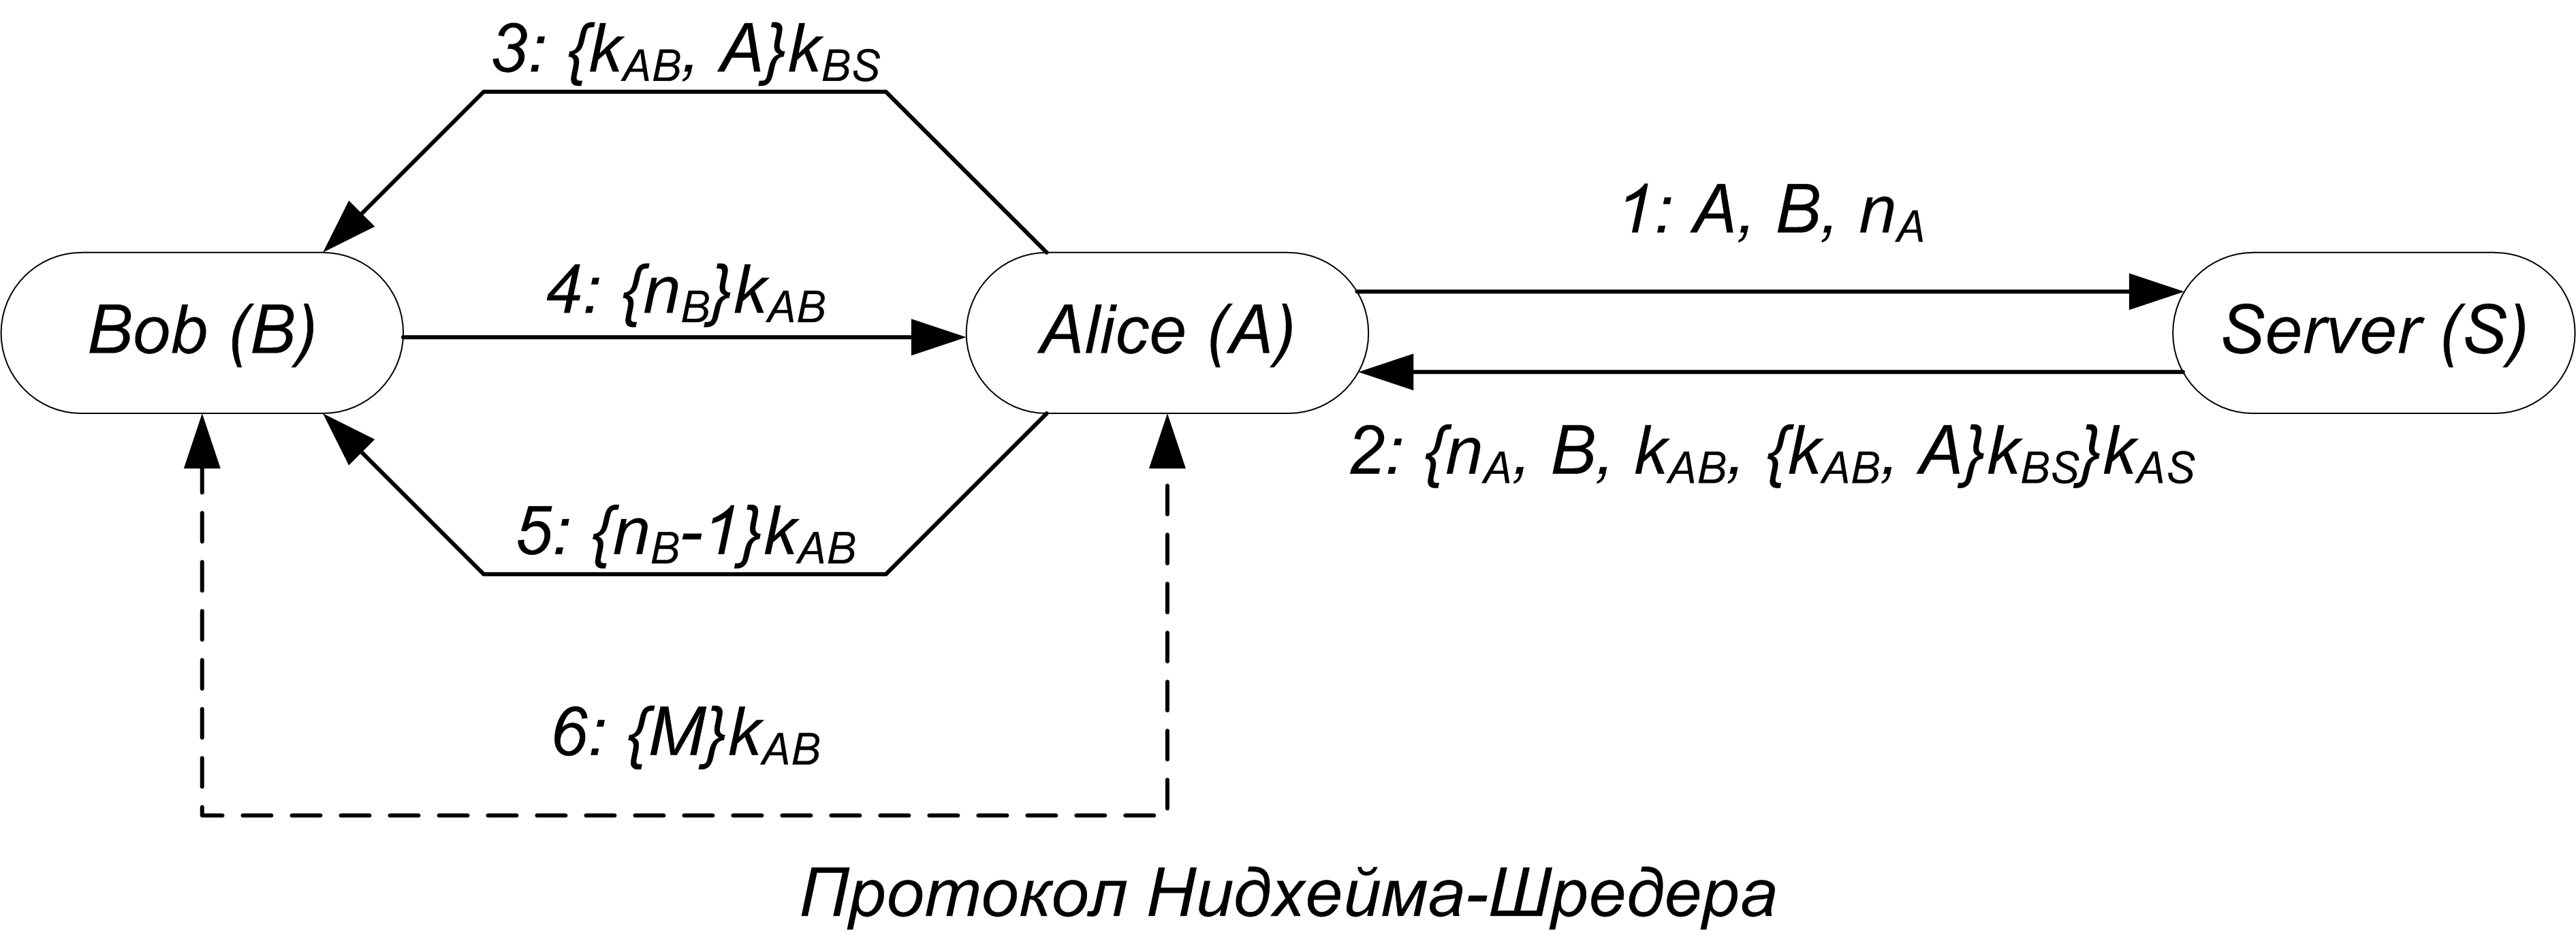
\includegraphics[width=.8\textwidth]{pict/nidhamshreder}  
                \caption{Протокол Нидхема-Шредера}\label{pict:nidhamshreder}
            }
        \end{center}
    \end{figure} 
    \mode<article>{см. рис. \ref{pict:nidhamshreder}}
\end{frame}

Недостатком протокола является то, что у абонента $B$ нет уверенности в том, что $k_{AB}$ новый! Злоумышленник, подобрав ключ предыдущих сеансов, может пройти фазы $3,4,5$ протокола, обманув $B$.

\begin{frame}
    \frametitle{Протокол Отвэй-Риса}
    
    \begin{figure}
        \begin{center}
            \mode<presentation>{ 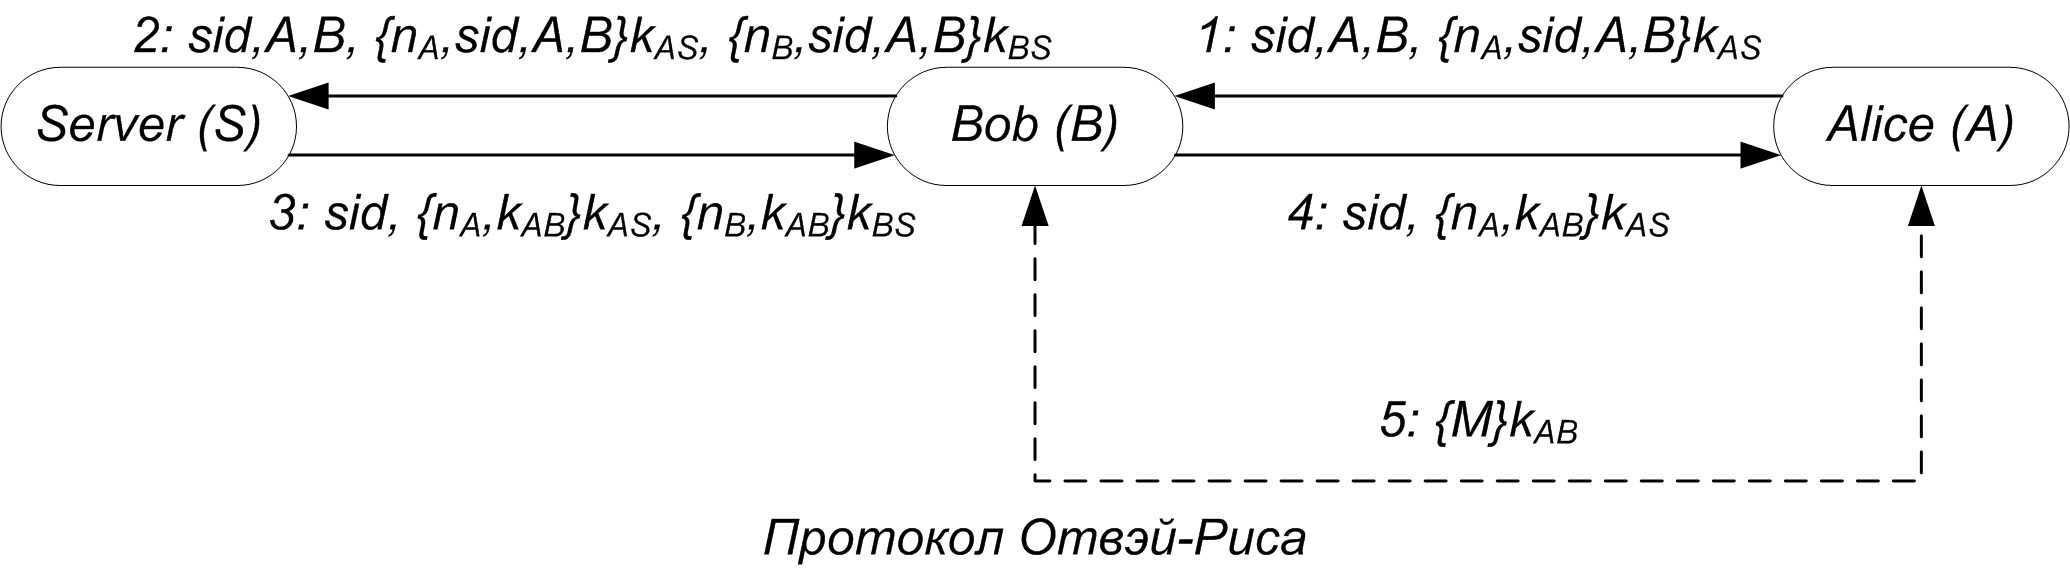
\includegraphics[width=.98\textwidth]{pict/otwayrease} }
            \mode<article>{ 
                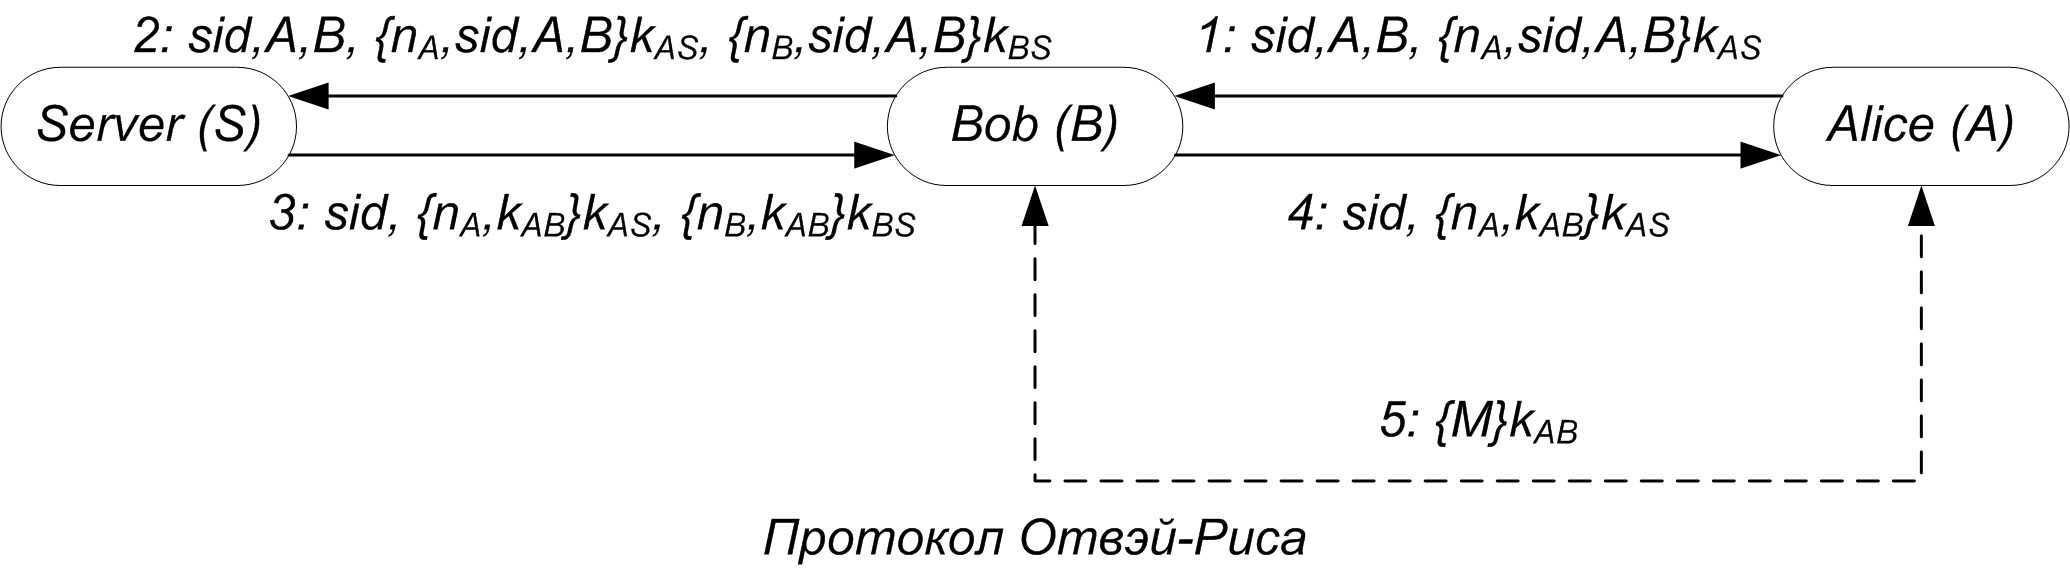
\includegraphics[width=.8\textwidth]{pict/otwayrease}  
                \caption{Протокол Отвэй-Риса}\label{pict:otwayrease}
            }
        \end{center}
    \end{figure} 
    \mode<article>{см. рис. \ref{pict:otwayrease}}
\end{frame}


\begin{frame}
    \frametitle{Протокол Kerberos v5}
    \framesubtitle{Первичный обмен ключами}
    
    \begin{figure}
        \begin{center}
            \mode<presentation>{ 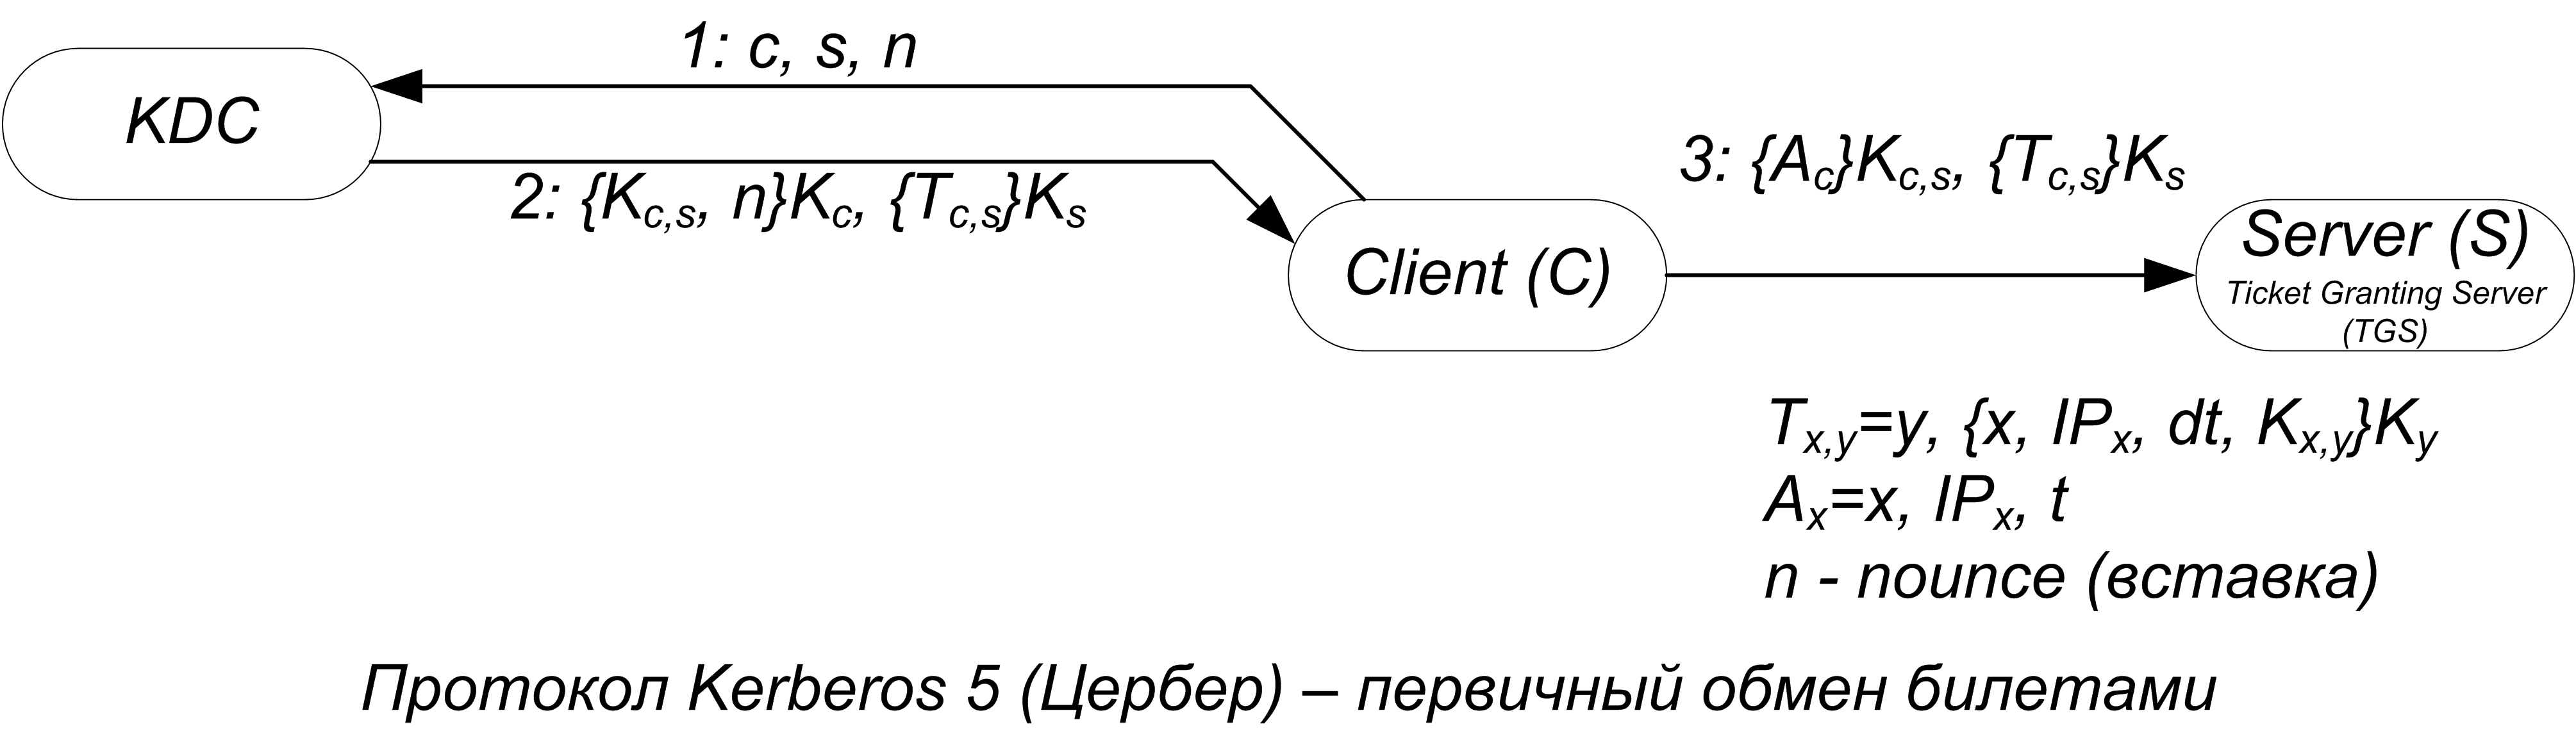
\includegraphics[width=.98\textwidth]{pict/kerberos1} }
            \mode<article>{ 
                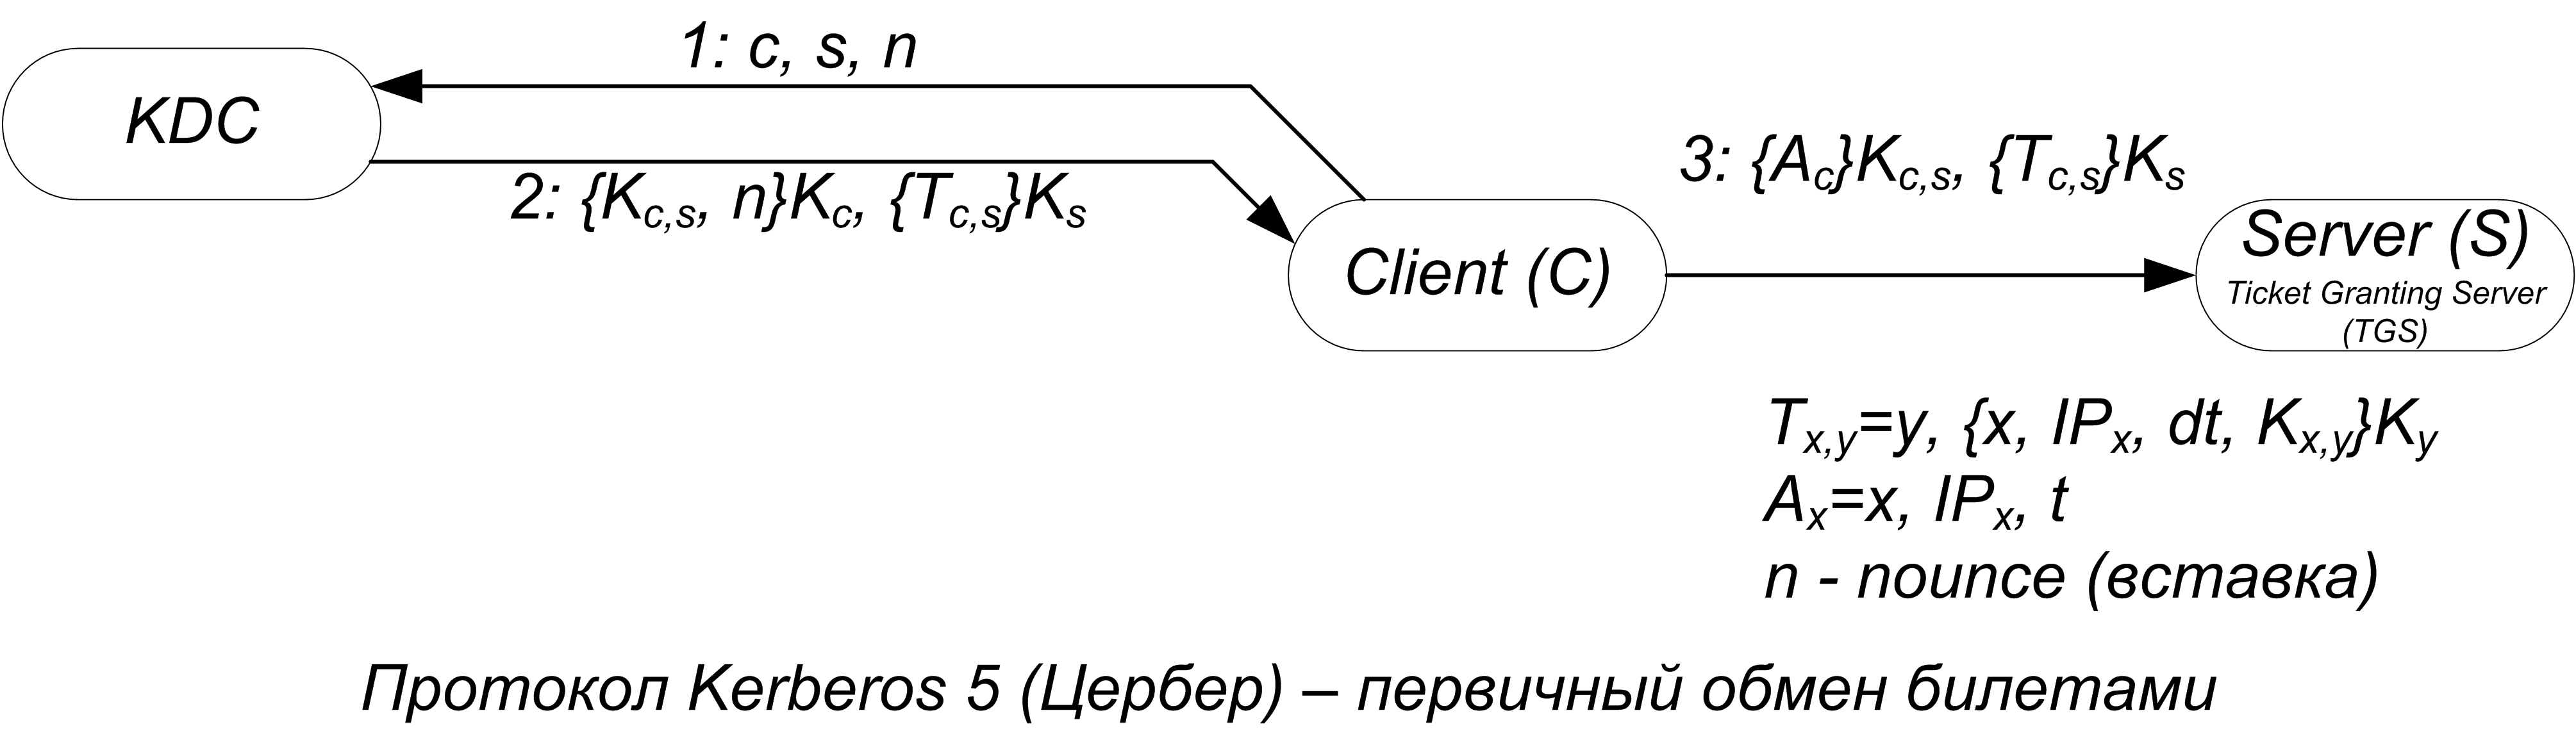
\includegraphics[width=.8\textwidth]{pict/kerberos1} 
                \caption{Протокол Kerberos v5}\label{pict:kerberos1}
            }
        \end{center}
    \end{figure} 
    \mode<article>{см. рис. \ref{pict:kerberos1}}
\end{frame}


\begin{frame}
    \frametitle{Протокол Kerberos v5}
    \framesubtitle{Полная схема обращения}
    
    \begin{figure}
        \begin{center}
            \mode<presentation>{ 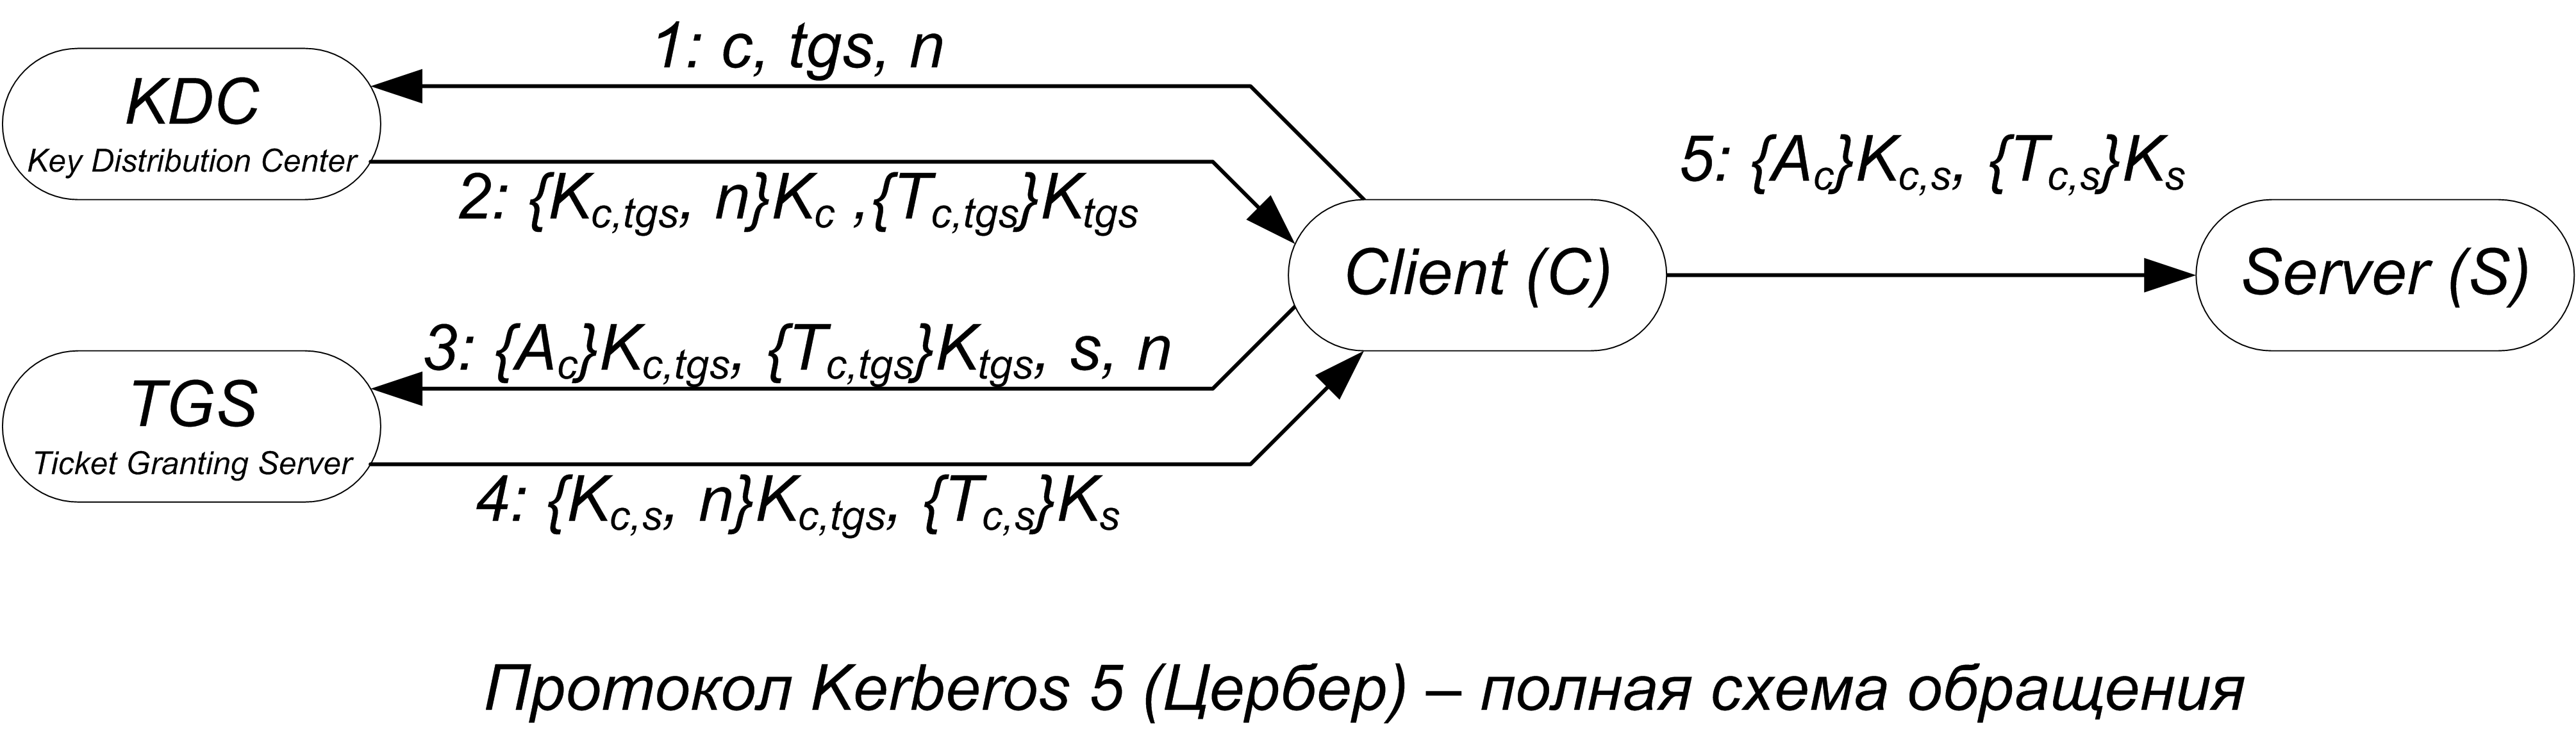
\includegraphics[width=.98\textwidth]{pict/kerberos2} }
            \mode<article>{ 
                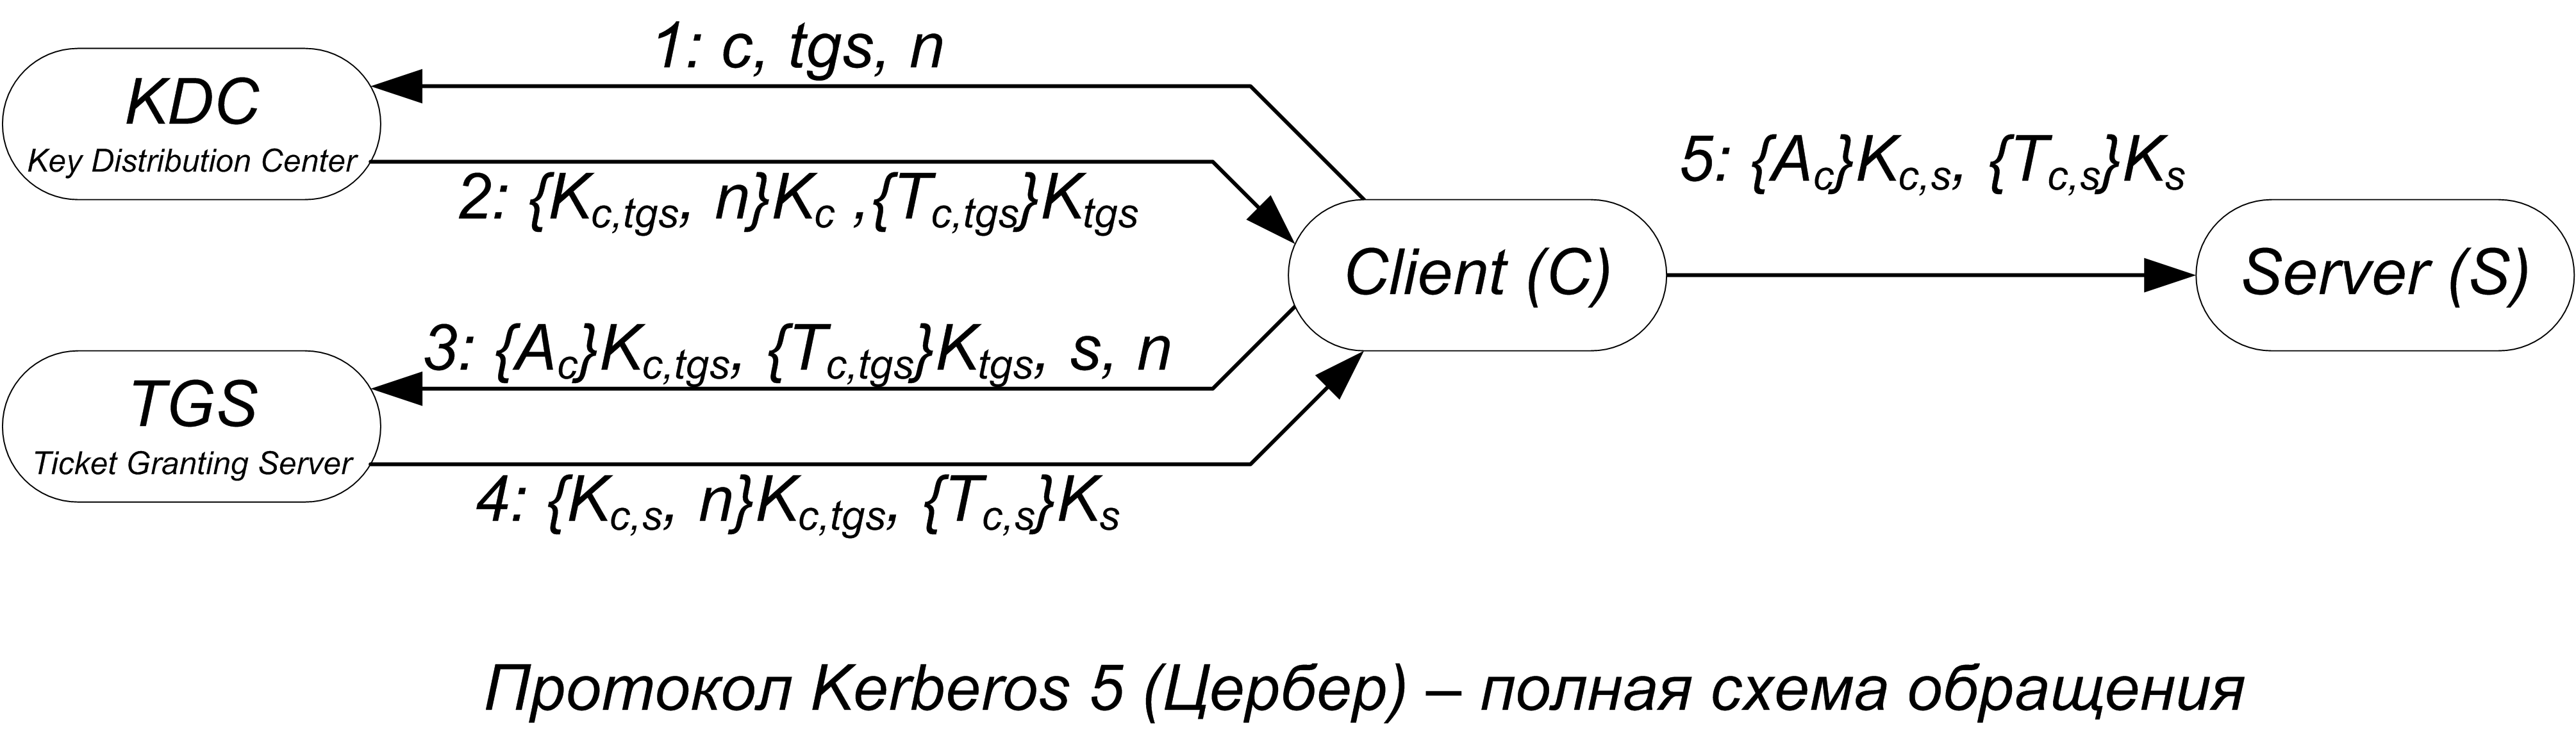
\includegraphics[width=.8\textwidth]{pict/kerberos2}  
                \caption{Протокол Kerberos v5}\label{pict:kerberos2}
            }
        \end{center}
    \end{figure} 
    \mode<article>{см. рис. \ref{pict:kerberos2}}
\end{frame}


\section{Протоколы распределения ключей асимметричной схемы}


\subsection{Ключи}


Особенности асимметричной схемы предполагают, что для безопасного обмена информацией между $n$ абонентами потребуется лишь $n$ пар ключей. Но схема требует аутентичного канала связи для передачи открытых ключей.

\begin{frame}
    \frametitle{Ключи}
    
    \begin{itemize}
        \item Общее количество пар ключей для безопасного обмена между $n$ абонентами составляет $n$.
        \item Для передачи открытых ключей требуетя \alert{аутентичный} канал связи.
        \item Для организации аутентичного канала применяется цифровая подпись\footnote{Для работы которой также требуется аутентичный канал. Такая рекурсия.} и схемы доверия, например сертификаты. Этот вопрос решается инфраструктурой открытого ключа PKI (Public Key Infrastructure), внедренной на предприятии.
        \item На практике для шифрования больших объемов данных используется сеансовый ключ симметричной схемы, который в свою очередь шифруется на открытом ключе.
    \end{itemize} 
\end{frame}


\subsection{Протокол обмена секретом Диффи-Хеллмана}


Рассмотрим в качестве примера применения арифметики остатков задачу обмена секретной информацией по общедоступному каналу связи. Двум абонентам $A$ и $B$ требуется безопасным образом передать секретное число, которе в дальнейшем может быть использовано, например, как ключ шифрования.

Предварительно абонентам следует обменяться некоторыми параметрами этого протокола, которые могут быть доступны всем желающим (общеизвестны), но у них  должна быть уверенность в том, что эти параметры не были подменены.

Итак, выбирается большое простое (512 и более бит\footnote{При современных вычислительных возможностях}) число $N$. При этом дополнительно накладываются ограничение: разложение $N-1$ на простые сомножители должно содержать по крайней мере один большой простой сомножитель. Также выбирается образующий\footnote{Образующим элементом называется элемент, степенью которого $a^i$ можно представить любой элемент кольца вычетов $\mathbb{Z}/N\mathbb{Z}$}.

Параметры протокола $a$, $N$ --- общеизвестны. Абоненты случайным образом генерируют \emph{секретные} ключи: абонент $A$ генерирует $x_A$, а абонет $B$ генерирует $x_B$. Секретный ключ известен только тому, кто его сгенерировал. Далее абоненты вычисляют соответствующие своим секретным ключам, \emph{открытые} ключи: абонент $A$ вычисляет $y_A\equiv a^{x_A}\pmod{N}$, а абонет $B$ вычисляет $y_B\equiv a^{x_B}\pmod{N}$. Открытые ключи $y_A, y_B$ также общедоступны (при условии, что их нельзя подменить).

Когда абоненты желают обменяться секретом (чаще всего это число-ключ, которое будет использовано для шифрования будущих сообщений\footnote{Сеансовый ключ}) они могут зашифровать его на фактически уже имеющемся у них <<общем>> ключе $S$.

Восстанавливается этот <<общий>> ключ следующим образом. 

Абонент $A$ знает параметры протокола $a$, $N$, открытый ключ абонента $B$ --- $y_B$ и собственный секретный ключ $x_A$, он вычисляет
\[S_A\equiv y_B^{x_A}\pmod{N}.\]

Абонент $B$ знает параметры протокола $a$, $N$, открытый ключ абонента $A$ --- $y_A$ и собственный секретный ключ $x_B$, он. вычисляет
\[S_B\equiv y_A^{x_B}\pmod{N}.\]

Но 
\[
S_A\equiv 
y_B^{x_A}\equiv 
a^{x_B\cdot x_A}\equiv 
a^{x_A\cdot x_B}\equiv 
y_A^{x_B}\equiv 
S_B\pmod{N}.
\]

Никто, кроме абонентов $A$ и $B$ сгенерировать $S=S_A=S_B$ не может. Так как для этого потребуется решить задачу дискретного логарифмирования.

\begin{frame}
    \frametitle{Протокол обмена секретом Диффи-Хеллмана}
    
    \begin{enumerate}
        \item Выбираются общие параметры протокола: большое простое число $N$ и образующий элемент $a$ поля $\mathbb{Z}/N\mathbb{Z}$. Каждый абонент случайным образом генерирует свой \alert{секретный} ключ: $x_A,x_B$.
        
        \item По \alert{аутентичному} каналу передаются открытые ключи $y_A,y_B$:
        \begin{itemize}
            \item $A\to B:y_A\equiv a^{x_A}\pmod{N}$
            \item $B\to A:y_B\equiv a^{x_B}\pmod{N}$
        \end{itemize}
        
        \item Теперь абоненты могут сгенерировать общий ключ $k$:
        \begin{itemize}
            \item $A:k_A\equiv y_B^{x_A}\pmod{N}$
            \item $B:k_B\equiv y_A^{x_B}\pmod{N}$
        \end{itemize}

        \[
        k\equiv k_A\equiv 
        y_B^{x_A}\equiv 
        a^{x_B\cdot x_A}\equiv 
        a^{x_A\cdot x_B}\equiv 
        y_A^{x_B}\equiv 
        k_B\pmod{N}.
        \]
        
        \item И организовать, например, обмен секретными сообщениями: \[\{M\}_k\] 
    \end{enumerate} 
\end{frame}


%TODO \subsection{Сертификаты, SSL/TLS}


\section{Пороговая $(m,n)$ схема разделения секрета}


Интересным примером является пороговая $(m,n)$ схема разделения секрета, когда из $m$ абонентов, разделяющих ключ, достаточно лишь любых $n$ из них ($n\leq m$) для восстановления ключа. Кусочек секрета, которым обладает отдельный участник разделения, называется \emph{слепком}.


\subsection{Задача об учёных}


\begin{frame}
    \frametitle{Задача об учёных}
    \framesubtitle{<<Жизненный>> пример пороговой $(m,n)$ схемы}
    
    \begin{example}
        Имеется $m$ ученых, один сейф и желание, чтобы $n$ ученых ($n\leq m$), собравшись вместе, смогли его открыть.
        Сколько замков нужно врезать в сейф и сколько ключей от этих замков раздать каждому участнику? 
    \end{example}
    
    \mode<presentation> {
        \uncover<2->{
            Замков: $\binom{m}{n-1}.$\\
            Ключей: $\binom{m-1}{n-1}.$\\
            Здесь $\binom{m}{n}=\frac{m!}{n!(m-n)!}$ --- количество сочетаний из $m$ по $n$
        }
    }
\end{frame}


В идеальном случае $n-1$ ученых, собравшись вместе, не смогут открыть всего один замок. Стало быть, каждая из возможных групп из $n-1$ ученых не сможет открыть некоторый <<свой>> замок (бессмысленно, если две разные группы не смогут открыть один и тот же замок --- это неидеальный случай). Следовательно, количество замков (и количество уникальных ключей) в сейфе:

\[ \binom{m}{n-1}, \]
где $\binom{m}{n}=\frac{m!}{n!(m-n)!}$ --- количество сочетаний из $m$ по $n$.

Ключ от $i$-го замка $k_i$ должны иметь $(m-n+1)$ ученых, так как $n-1$ участников не смогут открыть $i$-й замок, тогда как у каждого из остальных участников (коих количеством $m-(n-1)$) он не иначе как имеется!

Видно, что количество сочетаний групп участников должно дать количество уникальных ключей, то есть количество замков:
\[\binom{m}{m-n+1}.\]

Это действительно так, потому что \[\binom{m}{m-n+1}=\frac{m!}{(n-1)!(m-n+1)!}=\binom{m}{n-1}.\]

Количество замков определено и проверено. Далее, предполагая, что количество ключей у врачей одинаковое, общее количество ключей разделим на количество врачей:

\begin{multline*}
\frac{\binom{m}{n-1}(m-n+1)}{m}=
\frac{m!(m-n+1)}{m(n-1)!(m-n+1)!}=\\
=\frac{(m-1)!}{(n-1)!(m-n)!}=
\frac{(m-1)!}{(n-1)!((m-1)-(n-1))!}=
\binom{m-1}{n-1}
\end{multline*}

Таким образом, у каждого ученого имеется $\binom{m-1}{n-1}$ ключей, а каждый ключ принадлежит $m-n+1$ ученым (т.е. имеется $m-n+1$ копий каждого уникального ключа). Число уникальных ключей (замков) $\binom{m}{n-1}$ совпадает с количеством возможных раздач $m-n+1$ копий ключа среди $m$ ученых: $\binom{m}{m-n+1}$. Действительно $\binom{m}{n-1}=\frac{m!}{(n-1)!(m-n+1)!}=\binom{m}{m-n+1}$.

Стало быть имеем битовую матрицу: количество строк --- количество ключей ($k$), количество столбцов --- количество ученых ($s$). В строке ровно $m-n+1$ единиц, в столбце ровно $\binom{m-1}{n-1}$. В строках соответственно находятся все возможные варианты сочетаний $\binom{m}{m-n+1}$. Поэтому достаточно их все сгенерировать и все получится автоматически.

Построить число сочетаний $\binom{m}{n}$ можно перебрав двоичные числа $0\ldots 2^m-1$, отбросив числа, представление которых содержит единичные биты в количестве, не равном $n$.

Или воспользуйтесь рекурсией (см. табл.\ref{t:5to3scheme}):
\[
\binom{m}{n}=
\begin{cases}
    m, \text{если n=1. <<база:варианты с одной 1>>}\\
    1, \text{если n=m. <<база:все единицы>>}\\
    \sum_{i=n-1}^{m-1}\binom{i}{n-1},\text{если $m>n$. переход к базе}
\end{cases}
\]

Например, $(5,3)$ схема. Число замков (уникальных ключей) $\binom{5}{2}=10$. См. таблицу \ref{t:5to3scheme}.

\begin{frame}
    \frametitle{Пример $(5,3)$ схемы для задачи об учёных}
    \begin{table}[ht]
        \caption{$(5,3)$ пороговая схема для задачи об учёных}\label{t:5to3scheme}
        \centering
        \begin{tabular}[c]{|l||l|l|l|l|l|}
            \hline
                  & $s_1$ & $s_2$ & $s_3$ & $s_4$ & $s_5$\\ \hline\hline 
            $k_1$ &1&1&1&0&0\\ \hline 
            $k_2$ &1&1&0&1&0\\ \hline 
            $k_3$ &1&1&0&0&1\\ \hline 
            $k_4$ &1&0&1&1&0\\ \hline 
            $k_5$ &1&0&1&0&1\\ \hline 
            $k_6$ &1&0&0&1&1\\ \hline 
            $k_7$ &0&1&1&1&0\\ \hline 
            $k_8$ &0&1&1&0&1\\ \hline 
            $k_9$ &0&1&0&1&1\\ \hline 
            $k_{10}$&0&0&1&1&1\\ \hline 
        \end{tabular}
    \end{table}
\end{frame}


Пример: пусть ученых 11 человек, и необходимо, чтобы 6 и более ученых, собравшись вместе, открыли сейф. Замков $\binom{11}{5}=462$, ключей на каждого ученого $\binom{10}{5}=252$, копия каждого уникального ключа роздана $11-6+1=6$ ученым. Чудовищных размеров сейф для хранения одной пробирки и необходимость ежедневно носить около 5-и кило ключей (при среднем весе ключа 20 грамм) – уже подвиг ради науки!


\subsection{Пороговая $(m,n)$ схема Шамира}

Ключ $k$ разделяется на $m$ частей. По известным любым $n$ частям можно восстановить $k$.

\begin{frame}
    \frametitle{Схема Шамира}
    \framesubtitle{Формирование слепка}
    
    Выбирается большое простое число $P$. Доверенное лицо выбирает $m$ ненулевых значений $X_i\in GF(P), 1\leq i\leq m$. Каждый абонент $A_i$ знает свое $X_i$, а также и все остальные. Доверенное лицо выбирает \alert{секрет}: $n-1$ ненулевых элементов $a_j\in GF(P),1 \leq j\leq n-1$, а также ключ $k\in GF(P)$, и строит многочлен:

    \[F(X)\equiv k+\sum_{j=1}^{n-1}a_jX^j\pmod{P}.\]

    После этого доверенным лицом вычисляется $m$ значений $y_i = F(X_i)$ и раздаются соответствующим абонентам $A_i$. Ключ $k$ и элементы $a_j$ остаются в секрете.
\end{frame}

Доверенное лицо тут же распыляется на атомарные частички (только тогда ему можно по настоящему доверять!).

\begin{frame}
    \frametitle{Схема Шамира}
    \framesubtitle{Сборка секрета}

    Когда $L$ абонентов собираются вместе, они могут попытаться решить систему линейных уравнений:
    \[
        \begin{cases}
            y_{i_1}\equiv k+a_1X_{i_1}+\ldots+a_{n-1}X_{i_1}^{n-1}\pmod{P}\\
            y_{i_2}\equiv k+a_1X_{i_2}+\ldots+a_{n-1}X_{i_2}^{n-1}\pmod{P}\\
            \cdots\\
            y_{i_L}\equiv k+a_1X_{i_L}+\ldots+a_{n-1}X_{i_L}^{n-1}\pmod{P}
        \end{cases}
    \]

    Если $L\geq n$, то решить систему из $L$ уравнений при $n$ неизвестных ($k,a_1,a_2,\ldots,a_{n-1}$) можно. Иначе решений может быть очень много.
\end{frame}


\section{Жребий (залоговые схемы)}

\subsection{Подбрасывание монеты}

\begin{frame}
    \frametitle{Подбрасывание монеты}

    \begin{example}
        Абоненты $\Alice$ и $\Bob$ бросают жребий с помощью монеты. При этом они договорились о:
        \begin{enumerate}
            \item криптографической функции $H:M\to h$.
            \item соответствии 
            \(
                f(n)=
                \begin{cases}
                    \text{Орёл},    &\text{если $n$---чётное},\\
                    \text{Решка},   &\text{иначе}.
                \end{cases}
            \)
        \end{enumerate}
    \end{example}
    
    \uncover<2>{
        \begin{enumerate}
            \item\label{en:ch:ssplit:coin:hash} $\Alice\rightarrow\Bob:H(n_{\Alice})$. \alert{$\Alice$ подбрасывает монету.}
            \item $\Bob\rightarrow\Alice:f(n'_{\Alice})?$. 
                \alert{Попытка угадать.}
            \item $\Alice\rightarrow\Bob:n_{\Alice}$. \alert{$\Bob$ вычисляет $H(n_{\Alice})$ и сверяет с полученным на шаге \ref{en:ch:ssplit:coin:hash} значением, убеждаясь в правоте/неправоте своей догадки.}
        \end{enumerate}
    }
\end{frame}

\begin{frame}
    \frametitle{Розыгрыш на практике}

    \begin{example}
        \begin{enumerate}
            \item Угадай в какой руке?
            \item{} <<Камень, ножницы, бумага>>
            \item Загадал число\ldots
        \end{enumerate}
    \end{example}
\end{frame}


\appendix

\begin{frame}
    \frametitle{Источники}
    
    Протоколы распределения ключей симметричной схемы подробно рассмотрены в \cite{bib:smart:crypto}. Протокол Диффи-Хеллмана можно найти практически в любом, посвященном криптографии, издании \cite{bib:smart:crypto, bib:mao:modernCrypto, bib:shangin:protect}. Разделение секрета см. в \cite{bib:chmora:crypto,bib:smart:crypto}. Протоколы залоговой схемы см. в \cite{bib:mao:modernCrypto, bib:chmora:crypto}. Обзор специфичных протоколов безопасности (например, протоколы слепой подписи) см. в \cite{bib:shneir:applCrypto}.
\end{frame}


\begin{frame}[allowframebreaks]{Библиография}
    \bibliographystyle{gost780u}
    \bibliography{./../bibliobase}
\end{frame}


\end{document}